\section{Vorlesung 09.12.2016}
\subsection{Phylogenetische Kombinatorik}
		
\begin{itemize}
	\item Distanz Methoden / Clustering $\leftrightarrow$ Netzwerke statt Bäume 
	\item Supertree / Tripel-Methoden
\end{itemize}
\subsubsection{Phylogenetische Distanzen}

x = \color{red}0 \color{green}1 \color{red}1 \color{green}1 \color{red}0 \color{green}0 1\\\color{black}
y = \color{red}1 \color{green}1 \color{red}0 \color{green}1 \color{red}1 \color{green}0 1\\
\color{black}$\rightarrow$ Hamming Distanz: $d_h(x,y) = 3$

\begin{center}
	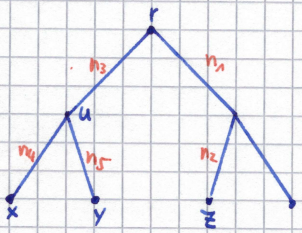
\includegraphics[scale=0.7]{lectures/161209/pix/evol_distanz}
\end{center}

Evolutionäre Distanz = Evol. Ereignisse; die x,y trennen	
\begin{align*}
	d_E (z,x) &= n_2 + n_1 + n_3 + n_4\\
	d_E (x,y) &= n_4 + n_5\\
	d_E (z,y) &= n_2 + n_1 + n_3 + n_5
\end{align*}
\begin{align*}
	d_E (z,x) &= d_E (z,u) + n_4\\
	d_E (z,y) &= d_E (z,u) + n_5\\
	d_E (z,x) + d_E (z,y) &= 2 d_E(z,u) + n_4 + n_5
\end{align*}
\begin{align*}
	d_E (z,u) &= \frac{1}{2} \lbrace d_E (z,x) + d_E (z,y) - d_E (x,y) \rbrace
\end{align*}

\begin{itemize}
	\item messbare Daten: Abstände zwischen Taxa $\equiv$ Blätter des Baumes
	\item Position der Wurzel:
		\begin{itemize}
			\item[*] jede messbare Distanz enthält entweder $(n_1 + n_3)$ oder weder $n_1$ noch $n_3$
			\item[*] genaue Position der Wurzel NICHT bestimmbar
			\item[$\rightarrow$] ungewurzelte Bäume
		\end{itemize}
\end{itemize}

\begin{center}
	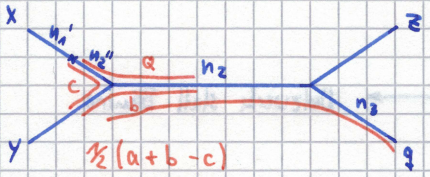
\includegraphics[scale=0.7]{lectures/161209/pix/ungew_baum}		
\end{center}

\begin{align*}
	d_H (x,y) &\leq d_E (x,y)
\end{align*}

\begin{center}
	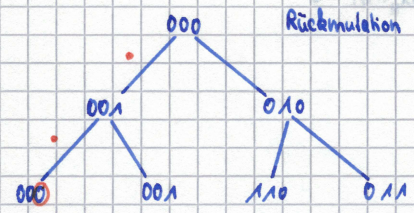
\includegraphics[scale=0.7]{lectures/161209/pix/gew_baum}
\end{center}

\newpage	

\subsubsection{Modell für Sep. Evolution}
\textbf{Markov:}
\begin{align*}
	P_{a,b}(\tau) &:= P(a | b, \tau) = \biggl[e^{\mu \tau R} \biggr]_{a,b}
\end{align*}

$\mu = $ Mutationsrate\\
$\tau = $ Zeit\\
$R = $ Matrix Mutationsmodell

\begin{align*}
	R = \begin{pmatrix}
		-1 & 1\\
		 1 &-1
	\end{pmatrix}
\end{align*}
\begin{align*}
	R = \begin{pmatrix}
		-3 & 1 & 1 & 1\\
		 1 &-3 & 1 & 1\\
		 1 & 1 &-3 & 1\\
		 1 & 1 & 1 &-3
	\end{pmatrix}
\end{align*}
\begin{align*}
	e^{\mu * \tau * R} &:= I + \tau * \mu * R + \frac{1}{2!} * \tau^2 * \mu^2 * R^2 + \frac{1}{3!} * \tau^3 * \mu^3 * R^3 + ...
\end{align*}
\begin{align*}
	P_{a,b}(\tau) &= \delta_{a,b} + \tau * \mu * R_{a,b} + ...
\end{align*}
a $=$ b:
\begin{align*}
	P_{a,a}(\tau) &= 1 + \tau * \mu * (-1) + \sigma (\tau ^2) = 1 - \tau * \mu + \sigma (\tau ^2)
\end{align*}
a $\neq$ b:
\begin{align*}
	P_{a,b}(\tau) &= 0 + \tau * \mu * 1 + \sigma (\tau ^2) = \tau * \mu + \sigma (\tau ^2)
\end{align*}

$\sigma (\tau ^2) = $ Rückmutation
 
\begin{center}
	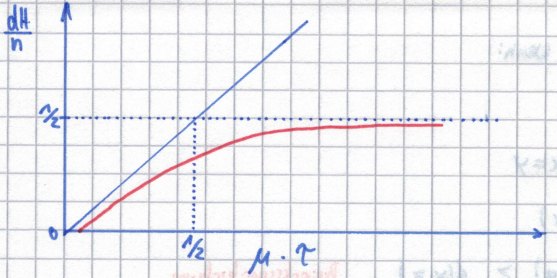
\includegraphics[scale=0.7]{lectures/161209/pix/diagramm}
\end{center}

\begin{align*}
	\frac{dH}{n}~=~P_{a,b} (\tau) | \{a \neq b\}~=~\tau * \mu + \sigma (\tau ^2)
\end{align*}
\begin{align*}
	\lim\limits_{\tau \rightarrow \infty} P_{a,b} (\tau)~=~ \frac{1}{2}
\end{align*}
\begin{align*}
 	\frac{dH}{n}~=~ \frac{1}{2} (1 - e^{-\tau * \mu})
\end{align*} 
$\frac{1}{2} =$ \color{orange} weil 2 Buchstaben\color{black}\\
$\tau * \mu =$ \color{orange} $dE$ \color{black}

\begin{align*}
 	dH(\tau) ~&=~ \sum \limits_{b \in A} \sum \limits_{a \neq b}  f_b^{Anfang} * P_{a,b}(\tau)\\
 	2 \frac{dH}{n} ~&=~ 1 - e^{-\tau * \mu}\\
 	e^{-\tau * \mu} ~&=~ 1 - 2 \frac{dH}{n}\\
 	\tau * \mu ~&=~ -ln (1 - 2 \frac{dH}{n}) = dE
\end{align*} 

\subsubsection{Evolutionäre Distanzen $\rightarrow$ Baum}
geg.: Baum T, Kantenlängen l: E(T) $\rightarrow \mathbb {R}_0^+$\\

\hspace{2cm} $\Rightarrow$ Distanzen $d(x,y) = \sum \limits_{e \in Pfad_T (x,y)} l(e)$ \color{orange}(*)\color{black}\\

\textbf{Definition:}\\
Eine metrische Distanz $d: X \times X \rightarrow \mathbb {R}_0^+$ \\
heißt ADDITIV, wenn es einen Baum T\\
mit Blättern X und Kantenlängen l gibt sodass \color{orange}(*)\color{black} stimmt	

Distanz heißt metrisch wenn:
\begin{itemize}
	\item[(i)] $d(x,x) = 0$
	\item[(ii)] $d(x,y) = 0 \rightarrow x = y$
	\item[(iii)] $d(x,y) = d(y,x)$
	\item[(iv)] $d(x,y) + d(y,z) \geq d(x,z)$
	\item \textcolor{orange}{für alle $x, y, z \in X$}
\end{itemize}

\newpage

\begin{itemize}
	\item[-] wann ist eine Distanz additiv?
\end{itemize}

Bem.: wenn $l(e) > 0$ für alle Kanten e $\Rightarrow$ additive Distanz ist metrisch

\begin{center}
	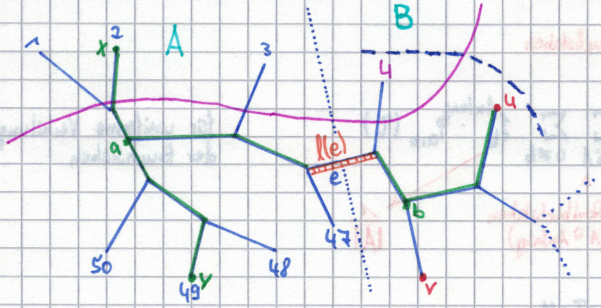
\includegraphics[scale=0.6]{lectures/161209/pix/distanz_metrisch}
\end{center}

Kante e induziert eine Partition von T und damit X in genau 2 Teilmengen, nicht leer \color{purple} SPLIT \color{black}

\begin{align*}
 	&A \cap B = \emptyset \\
 	&A \neq 0 \\
 	&B \neq 0 \\
 	&A \cup B = X
\end{align*}
Sei A | B der Split, der zu e gehört\\
$x,y \in A$\\
$u,v \in B$\\

\begin{center}
	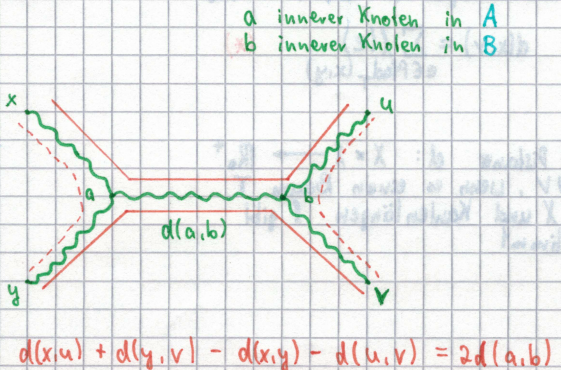
\includegraphics[scale=0.6]{lectures/161209/pix/split}
\end{center}

\newpage

\begin{center}
	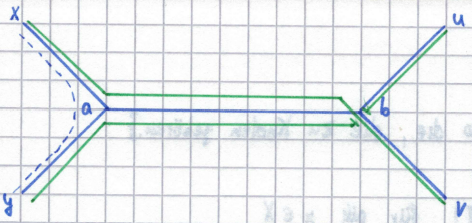
\includegraphics[scale=0.6]{lectures/161209/pix/split_two}
\end{center}

\begin{align*}
 	d(x,y) + d(y,u) - d(x,y) - d(u,v) = 2 d(a,b)\\
 	l(e) = min_{x,y \in A; u,v \in B} d(x,u) + d(y,v) - d(x,y) - d(u,v)
\end{align*} 

\begin{itemize}
	\item[-] was wenn A, B nicht zu einer Kante gehören?
\end{itemize}

\begin{center}
	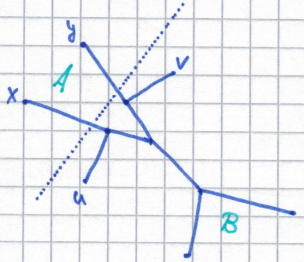
\includegraphics[scale=0.6]{lectures/161209/pix/kante}
\end{center}

\begin{center}
	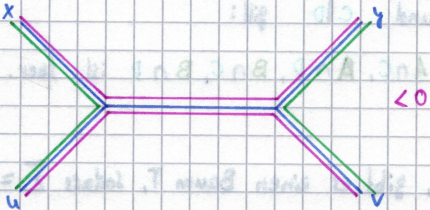
\includegraphics[scale=0.6]{lectures/161209/pix/split_three.png}
\end{center}

wenn A | B kein Split von T $\Rightarrow l(A|B) < 0$\\
wenn A | B Split von T $\Rightarrow l(A|B) = l(e)$ 

\begin{align*}
 	l(A|B) = \frac{1}{2} min_{x,y \in A; u,v \in B} d(x,u) + d(y,v) - d(x,y) - d(u,v)
\end{align*}

\newpage

für je 4 Blätter betrachte:\\
\begin{align*}
 	d(x,u) + d(y,v) - d(x,y) - d(u,v)\\
 	d(x,v) + d(y,u) - d(x,y) - d(u,v)\\
 	d(x,y) + d(u,v) - d(x,u) - d(y,v)
\end{align*}
2 dieser 3 Summen sind gleich, die 3te ist nicht größer.\\

\subsubsection{Splitsystem eines Baums}

$\sum (T) = \{$ splits in T, also die, die zu Knoten gehören. $\}$

\begin{enumerate}
	\item[1)] $ \{ x \}~|~X \setminus \{ x \} \in \sum (T)$ für alle $x \in X$
\end{enumerate}

\begin{center}
	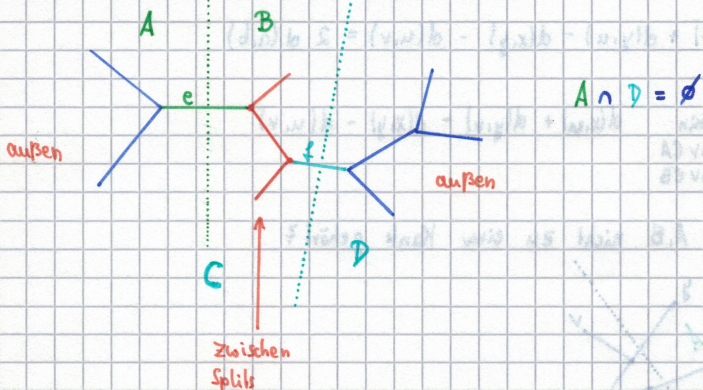
\includegraphics[scale=0.6]{lectures/161209/pix/splitsystem}
\end{center}

$\sum$ heißt KOMPATIPEL, wenn \\
für zwei Splits A | B und C | D gilt:\\
mindestens ein Durchschnitt $A \cap C$, $A \cap D$, $B \cap C$, $B \cap D$ ist leer.\\

Satz: Wenn $\sum$ kompatibel, gibt es einen Baum T, sodass $\sum = \sum(T)$